%
% fluiddynamik.tex
%
% (c) 2018 Prof Dr Andreas Müller, Hochschule Rapperswil
%
\chapter{Fluiddynamik\label{chapter:fluiddynamik}}
\lhead{Fluiddynamik}
\rhead{}
Die Atmosphäre und die Ozeane unterschieden sich in ihren
für das Studium von Wetter und Klima wesentlichen Eigenschaften
ganz beträchtlich.
Das Wasser der Ozeane ist fast inkompressibel, seine Dichte hängt aber
von der Temperatur und dem Salzgehalt ab.
Wasser hat eine sehr grosse Wärmekapazität, ausserdem kann Wärme durch
Verdunstung aus den Ozeanen in die Atmosphäre übergehen, wobei gleichzeigit
die Salzkonzentration steigt.

Die Atmosphäre auf der anderen Seite hat eine wesentlich geringere
Dichte und Wärmekapazität, ihre Temperatur kann sich daher sehr viel
schneller ändern.
Sie ist stark kompressibel.
Wegen der geringeren Dichte kann die Atmosphäre sehr viel höhere
Strömungsgeschwindigkeiten erreichen.

Trotz dieser grossen Unterschiede lassen sich Atmosphäre und Ozeane
beide als Fluide mit den gleichen partiellen Differentialgleichungen
beschreiben, die im folgenden hergeleitet werden sollen.
Die Unterschiede äussern sich vor allem in den Zustandsgleichungen,
die die Zustandsgrössen Druck, Temepratur, Dichte und Saltzgehalt
miteinander in Beziehung setzen.
Im ersten Abschnitt dieses Kapitels sollen die Grundgleichungen
der Fluiddynamik zusammengestellt werden.
Im zweiten Teil wird am Beispiel des Lorenz-Systems gezeigt, dass
die Gleichungen der Fluiddynamik trotzdem nur beschränkt eine exakte
Prognose des Wetters gestatten können.

%
% hydrodynamik.texo
%
% (c) 2018 Prof Dr Andreas Müller, Hochschule Rapperswil
%
\section{Fluiddynamik}
\rhead{Fluiddynamik}
%Die Atmosphäre und die Ozeane unterschieden sich in ihren
%für das Studium von Wetter und Klima wesentlichen Eigenschaften
%ganz beträchtlich.
%Das Wasser der Ozeane ist fast inkompressibel, seine Dichte hängt aber
%von der Temperatur und dem Salzgehalt ab.
%Wasser hat eine sehr grosse Wärmekapazität, ausserdem kann Wärme durch
%Verdunstung aus den Ozeanen in die Atmosphäre übergehen, wobei gleichzeigit
%die Salzkonzentration steigt.
%
%Die Atmosphäre auf der anderen Seite hat eine wesentlich geringere
%Dichte und Wärmekapazität, ihre Temperatur kann sich daher sehr viel
%schneller ändern.
%Sie ist stark kompressibel.
%Wegen der geringeren Dichte kann die Atmosphäre sehr viel höhere
%Strömungsgeschwindigkeiten erreichen.
%
%Trotz dieser grossen Unterschiede lassen sich Atmosphäre und Ozeane
%beide als Fluide mit den gleichen partiellen Differentialgleichungen
%beschreiben, die im folgenden hergeleitet werden sollen.
%Die Unterschiede äussern sich vor allem in den Zustandsgleichungen,
%die die Zustandsgrössen Druck, Temepratur, Dichte und Saltzgehalt
%miteinander in Beziehung setzen.
%
In diesem Abschnitt gehen wir davon aus, dass das Fluid beschrieben wird
durch Funktionen der Raumkoordinaten $(x,y,z)$ und der Zeit $t$,
wobei wir meistens darauf verzichten, die unabhängigen Variablen
auszuschreiben.
Die Temperatur $T$ ist also zu lesen als die Funktion $T(x,y,z,t)$.
Die Newtonschen Bewegungsgleichungen stellen eine Verbindung zwischen
Masse, Beschleunigung und Kraft her, wir können daher davon ausgehen,
dass die Bewegungsgleichungen eines Fluides nur die Dichte $\varrho$ und 
den Geschwindigkeitsvektor $\vec{v}$ involvieren.
Den Zusammenhang zwischen Druck, Temperatur, Dichte und möglicherweise
weiteren Eigenschaften wird durch Zustandsgleichungen vermittelt.

\subsection{Kontinuitätsgleichung}
Die Kontinuitätsgleichung drückt aus, dass
Materie nicht einfach neu entstehen oder verschwinden kann.
Um sie herzuleiten, betrachten wir ein Volumen $V$ des Fluids.
Die Masse im Inneren des Volumens wird bestimmt durch das Volumenintegral
\[
m
=
\iiint_V \varrho \,dx\,dy\,dz.
\]
Ein kleiner Quader mit den Abmessungen $\Delta x$, $\Delta y$
und $\Delta z$ enthält die Masse 
\[
m = \varrho \Delta x \,\Delta y \, \Delta z.
\]
Wenn sich die Masse in dem Quader ändert, dann muss Materie durch die
Wände zu- oder abfliessen.
Wir berechnen daher für jede Wand des Quaders, wie gross der Massefluss
durch die Wand in einer Zeiteinheit $\Delta t$ ist.

Durch ein Rechteck mit Abmessungen $\Delta y \times \Delta z$ senkrecht
zur $x$-Achse fliesst in der Zeit $\Delta t$ das Volumen
$v_x\Delta x\,\Delta y\,\Delta z$ und damit die Masse
\begin{equation}
\varrho v_x\,\Delta y\,\Delta z.
\label{skript:massenausdruck}
\end{equation}
Die Dichte $\varrho$ und die Geschwindigkeit $v_x$ sind dabei an der
Koordinate $x$ zu nehmen.
Durch die Wand des Quaders bei $x+\Delta x$ fliesst eine Masse, die
ebenfalls durch den Ausdruck \eqref{skript:massenausdruck}
beschrieben werden kann, jedoch für die $x$-Koordinaten $x+\Delta x$.
Um die Massenänderung im Quader zu bestimmen, sind diese beiden Ausdrücke
als mit entgegengesetzten Vorzeichen zu berücksichtigen.

Die Massenänderung ist daher
\begin{align}
\Delta m
&=
\varrho(x,y,z,t) v_x(x,y,z,t)\,\Delta y\,\Delta z\,\Delta t
-
\varrho(x+\Delta x,y,z,t) v_x(x+\Delta x,y,z,t)\,\Delta y\,\Delta z\,\Delta t
\notag
\\
&\quad
+
\varrho(x,y,z,t) v_y(x,y,z,t)\,\Delta x\,\Delta z\,\Delta t
-
\varrho(x,y+\Delta y,z,t) v_y(x,y+\Delta y,z,t)\,\Delta x\,\Delta z\,\Delta t
\notag
\\
&\quad
+
\varrho(x,y,z,t) v_z(x,y,z,t)\,\Delta x\,\Delta y\,\Delta t
-
\varrho(x,y,z+\Delta z,t) v_z(x,y,z+\Delta z,t)\,\Delta x\,\Delta y\,\Delta t.
\notag
\intertext{Wir fassen die Terme zu gegenüberliegenden Wänden zusammen wobei
wir das Produkt $\Delta x\,\Delta y\,\Delta z$ ausklammern können.
Wir teilen ausserdem durch $\Delta t$, um die zeitliche Massenänderungsrate
zu erhalten.}
\frac{\Delta m}{\Delta t}
&=
-
\bigg(
\frac{\varrho(x+\Delta x,y,z,t)v_x(x+\Delta x,y,z,t)-\varrho(x,y,z,t)v_x(x,y,z,t)}{\Delta x}
\notag
\\
&\qquad
+\frac{\varrho(x,y+\Delta y,z,t)v_y(x,y+\Delta y,z,t)-\varrho(x,y,z,t)v_y(x,y,z,t)}{\Delta y}
\notag
\\
&\qquad
+\frac{\varrho(x,y,z+\Delta z,t)v_y(x,y,z+\Delta z,t)-\varrho(x,y,z,t)v_y(x,y,z,t)}{\Delta z}
\bigg)
\Delta x\,\Delta y\,\Delta z\,\Delta t.
\notag
\intertext{Da $\Delta m=\varrho\Delta x\,\Delta y\,\Delta z$ können wir
auf beiden Seiten durch $\Delta x\,\Delta y\,\Delta z$ dividieren.
Um die zeitliche Änderung zu bestimmen, müssen wir ausserdem durch
$\Delta t$ dividieren.
Lassen wir die Inkremente $\Delta x$, $\Delta y$, $\Delta z$ und
$\Delta t$ gegen $0$ gehen, werden aus den Differenzenquotienten
Ableitungen.
Wir erhalten daher die {\em Kontinuitätsgleichung}
\index{Kontinuitätsgleichung} }
\frac{\partial \varrho}{\partial t}
&=
-
\biggl(
\frac{\partial \varrho v_x}{\partial x}
+
\frac{\partial \varrho v_y}{\partial y}
+
\frac{\partial \varrho v_z}{\partial z}
\biggr).
\label{skript:kontinuitaetsgleichung}
\end{align}
\index{Kontinuitätsgleichung}%
Die rechte Seite kann mit Hilfe des {\em Nabla-Operators}
\index{Nabla-Operator}
\[
\nabla
=
\begin{pmatrix}
\frac{\partial}{\partial x}\\
\frac{\partial}{\partial y}\\
\frac{\partial}{\partial z}
\end{pmatrix}
\]
kürzer geschrieben werden.
Der Nabla-Operator wird wie ein Vektor behandelt.
Für eine (skalare) Funktion $f$ ist $\nabla f$ ein Vektor,
der {\em Gradient}
\index{Gradient} der Funktion $f$.
Das Skalarprodukt $\nabla\cdot\vec{v}$ ist ein Skalar, die
{\em Divergenz}
\index{Divergenz}
eines Vektorfeldes $\vec{v}$, sie wird manchmal auch 
$\operatorname{div}\vec{v}$ geschrieben.
Aus 
\eqref{skript:kontinuitaetsgleichung}
wird dann
\[
\frac{\partial \varrho}{\partial t}
=
-\nabla\cdot (\varrho\vec{v})
\]
geschrieben werden.
%So erhält die Kontinuitätsgleichung die kompakte Form
%\[
%\frac{\partial}{\partial t}\varrho = -\nabla\cdot (\varrho\vec{v}).
%\]

\subsection{Inkompressible Strömung}
Bei einem inkompressiblen Fluid ist die Dichte eine Konstante, alle
\index{Fluid!inkompressibel}
\index{inkompressibel}
Ableitungen von $\varrho$ verschwinden.
Die Kontinuitätsgleichung wird damit zu
\[
\frac{\partial\varrho}{\partial t}
=
-\nabla\cdot(\varrho\vec{v})
=
-\nabla\varrho\cdot\vec{v}
-\varrho\nabla\vec{v}
=
-\varrho\nabla\vec{v}
=
0.
\]
In einer inkompressiblen Strömung verschwindet daher die Divergenz
des Geschwindigkeitsfeldes.

\subsubsection{Verallgemeinerung}
Die Herleitung der Kontinuitätsgleichung für die Massedichte funktioniert
auch für jede andere Erhaltungsgrösse, die im Fluid mit einer Dichte
$a(x,y,z,t)$ vorhanden ist und mit der Strömung mittransportiert wird.
Die {\em verallgemeinerte Kontinuitätsgleichung} für die Erhaltungsgrösse $a$
\index{Kontinuitätsgleichung!verallgemeinerte}
ist daher
\begin{equation}
\frac{\partial a}{\partial t}
=
-
\nabla(a\vec{v}).
\label{skript:verallgemeinerte kontinuitaetsgleichung}
\end{equation}

\subsection{Bewegungsgleichung}
Das zweite Newtonsche Gesetz $F=ma$ besagt, dass Kraft und Beschleunigung
proportional sind.
Dies gilt jedoch nur, wenn die Masse unveränderlich ist.
Genauer besagt Newtons zweites Gesetz, dass die Kraft die
zeitliche Änderung des Impulses ist, also
\[
F=
\frac{d}{dt}(m\vec v).
\]
Ein Volumen des Fluides kann wegen veränderlicher Dichte seine
Masse verändern.
Kräfte auf das Fluid ändern daher die Impulsdichte des Fluids.

\subsubsection{Impulsdichte}
Die Impulsdichte des Fluids wird an jeder Stelle durch die Grösse
$\vec{p}=\varrho\vec{v}$ gegeben.
Das zweite Newtonsche Gesetz besagt dann, dass die Änderung von $\vec p$
durch die äusseren Kräfte $\vec{b}$ bestimmt wird, die auf das Fluid wirkt.
Der Impuls in einem Volumen kann aber auch ändern, dass das Fluid Impuls
in das Volumen hinein- oder aus dem Volumen heraustransportiert.
Jede Komponente des Impulses ist eine Erhaltungsgrösse, für die ohne
Wirkung äusserer Kräfte die verallgemeinerte Kontinuitätsgleichung
\eqref{skript:verallgemeinerte kontinuitaetsgleichung}
gilt.
Für die $x$-Komponente des Impulses gilt daher die Gleichung
\[
\frac{\partial \varrho v_x}{\partial t}
=
-\nabla \cdot(\varrho v_x\,\vec{v})
+\varrho b_x,
\]
und analog für die anderen Komponenten $\varrho v_y$ und $\varrho v_z$ 
der Impulsdichte.

\subsubsection{Innere Kräfte}
Damit sind aber innere Kräfte im Fluid noch nicht berücksichtigt.
Das Fluid widersetzt sich zum Beispiel der Kompression, dies äussert
sich im Druck, der jeweils senkrecht auf den Wänden des Volumens wirkt.
In einem zähen Medium sind aber auch Kräfte parallel zu den Wänden
\index{Zähigkeit}
möglich, sogenannte {\em Scherkräfte}.
\index{Scherkraft}
Im Allgemeinen wirkt auf ein $\Delta y\times\Delta z$-Rechteck senkrecht
zur $x$-Achse die Kraft
\[
\vec{\tau}_x
\,\Delta y\,\Delta z
=
\begin{pmatrix}
\tau_{xx}\\
\tau_{xy}\\
\tau_{xz}
\end{pmatrix}
\,\Delta y\,\Delta z
\]
und analog für die Wände senkrecht auf der $y$- bzw.~$z$-Achse.
Die diagonalen Komponente $\tau_{ii}$ beschreiben die Druckkraft
\index{Druck}
auf die jeweilige Seitenfläche, während die ausserdiagonalen Elemente
Scherkräfte beschreiben.

Die Matrix $\bm{\tau}$ mit Komponenten $\tau_{ij}$ heisst auch der
{\em Cauchy-Spannungstensor}.
\index{Cauchy-Spannungstensor}
\index{Spannungstensor}
Wir werden weiter unten (Seite~\pageref{skript:spannungstensor symmetrisch})
zeigen, dass $\tau_{ij}$ symmetrisch sein muss,
Dass $\tau_{ij}$ ein Tensor ist, ist für die weiteren Erörterungen nicht
von Bedeutung, wir werden daher diesen Begriff verwenden, ohne ihn wirklich
zu definieren.

Die resultierende Kraft $\vec{F}$ auf einen Quader mit den Kantenlängen
$\Delta x$, $\Delta y$ und $\Delta z$  hat daher die $i$-Komponente
\begin{align*}
F_x
&=
(
\tau_{xx}(x+\Delta x,y,z,t)
-
\tau_{xx}(x,y,z,t)
) \Delta y\,\Delta z
\\
&\qquad
+
(
\tau_{yx}(x,y+\Delta y,z,t)
-
\tau_{yx}(x,y,z,t)
) \Delta x\,\Delta z
\\
&\qquad
+
(
\tau_{zx}(x,y,z+\Delta z,t)
-
\tau_{zx}(x,y,z,t)
)\Delta x\,\Delta z
\\
&=
\bigg(
\frac{
\tau_{xx}(x+\Delta x,y,z,t)
-
\tau_{xx}(x,y,z,t)
}{\Delta x}
+
\frac{
\tau_{yx}(x,y+\Delta y,z,t)
-
\tau_{yx}(x,y,z,t)
}{\Delta y}
\\
&\qquad
+
\frac{
\tau_{zx}(x,y,z+\Delta z,t)
-
\tau_{zx}(x,y,z,t)
}{\Delta z}
\bigg)
\Delta x\,\Delta y\,\Delta z.
\end{align*}
Die Kraftdichte $f_i$ erhalten wir nach Division durch
$\Delta x\,\Delta y\,\Delta z$ und Grenzübergang, sie ist
\begin{equation}
f_x
=
\frac{\partial \tau_{xx}}{\partial x}
+
\frac{\partial \tau_{yx}}{\partial y}
+
\frac{\partial \tau_{zx}}{\partial z}.
\label{skript:spannungskraftdichte}
\end{equation}
Wir können damit die vollständige Bewegungsgleichung für das Fluid
hinschreiben, sie lautet
\begin{equation}
\frac{\partial \varrho v_x}{\partial t}
=
-\nabla\cdot (\varrho v_x\vec{v})
+
\varrho b_x
+
f_x.
\label{skript:navier-stokes komponente}
\end{equation}
\subsubsection{Vektorschreibweise}
Die Schreibweise
\eqref{skript:navier-stokes komponente}
für die Bewegungsgleichungen ist sehr schwerfällig und passt nicht
zu der deutlich elegantere vektoriellen Schreibweise zum Beispiel
der Kontinuitätsgleichung.
Die linke Seite von
\eqref{skript:navier-stokes komponente}
und der mittlere Term auf der rechten Seite können natürlich sofort
in eine vektorielle Schreibweise überführt werden, nicht jedoch die
anderen zwei Terme.

Der Term $\nabla \cdot(\varrho v_x\vec{v})$ ist ausgeschrieben
\[
\nabla \cdot(\varrho v_x\vec{v})
=
\frac{\partial}{\partial x}
(\varrho v_xv_x)
+
\frac{\partial}{\partial y}
(\varrho v_xv_y)
+
\frac{\partial}{\partial z}
(\varrho v_xv_z).
\]
Dieser Ausdruck sieht ganz ähnlich aus wie der Ausdruck
\eqref{skript:spannungskraftdichte}
für die $x$-Kompontente der Kraftdichte der inneren Kräfte.
Wir können die Ähnlichkeit formal noch etwas klarer machen.
Schreiben wir $A_{xy} = \varrho v_xv_y$, dann ist
\[
\nabla \cdot(\varrho v_x\vec{v})
=
\frac{\partial A_{xx}}{\partial x}
+
\frac{\partial A_{xy}}{\partial y}
+
\frac{\partial A_{xz}}{\partial z}
=
\sum_{i}\frac{\partial A_{xi}}{\partial i}.
\]
Da es offenbar auf die Reihenfolge der Indizes von $A$ nicht ankommt,
ist dies auch das gleiche wie
\[
\nabla \cdot(\varrho v_x\vec{v})
=
\frac{\partial A_{xx}}{\partial x}
+
\frac{\partial A_{yx}}{\partial y}
+
\frac{\partial A_{zx}}{\partial z}
=
\sum_{i}\frac{\partial A_{ix}}{\partial i}.
\]
Wir können daher die Wirkung des Nabla-Operators $\nabla$ auf einer
symmetrischen Matrix $A$ wie folgt definieren:

\begin{definition}
\label{skript:definition divergenz}
\index{Divergenz!einer Matrix}
Ist $A_{ij}$ eine symmetrische Matrix, dann ist die {\em Divergenz}
$\nabla\cdot A$
von
$A$ der Vektor mit den Komponenten
\[
(\nabla\cdot A)_x
=
\sum_{i}\frac{\partial A_{ix}}{\partial i}.
\]
\end{definition}
Falls die Matrix $\tau_{ij}$ symmetrisch ist, kann diese Definition
auch auf $\bm{\tau}$ angewendet werden.
Die $x$-Komponente der Divergenz von $\bm{\tau}$ ist dann
\[
(\nabla\cdot \bm{\tau})_x
=
\frac{\partial \tau_{xx}}{\partial x}
+
\frac{\partial \tau_{yx}}{\partial y}
+
\frac{\partial \tau_{zx}}{\partial z}
=
f_x.
\]
Dies ist genau der letzte Term in der Gleichung
\eqref{skript:navier-stokes komponente}.

Wir brauchen jetzt nur noch eine kompaktere Notation für die Matrix
$\varrho v_xv_y$.

\begin{definition}
\index{Kronecker-Produkt}
Das {\em Kronecker-Produkt} zweier Vektoren $\vec{a}$ und $\vec{b}$ ist die
Matrix $\vec{a}\otimes\vec{b}=\vec{a}\vec{b}^t$ mit den Komponenten
\[
(\vec{a}\otimes\vec{b})_{ij}
=
a_ib_j
=
(
\vec{a}
\vec{b}^t
)_{ij}
\]
Abgekürzt erlauben wir die Schreibweise $\vec{a}\otimes\vec{b}=\vec{a}\vec{b}$.
\end{definition}

Mit diesen Notationen bekommen wir jetzt die Bewegungsgleichungen in
Vektorform.
Sie lauten
\begin{equation}
\frac{\partial \varrho\vec v}{\partial t}
=
-\nabla\cdot(\varrho\vec{v}\vec{v})
+ \varrho\vec{b}
+ \nabla\cdot \bm{\tau}.
\label{skript:navier-stokes1}
\end{equation}
Dies ist die {\em Navier-Stokes Gleichung}.
\index{Navier-Stokes Gleichung}
Die drei Terme beschreiben die Impulsänderung durch den Zu- oder Abtransport
von Impuls durch die Strömung, durch die äusseren Kräfte bzw.~die inneren
Spannungen.

\subsubsection{Symmetrie des Spannungstensors}
\label{skript:spannungstensor symmetrisch}
\begin{figure}
\centering
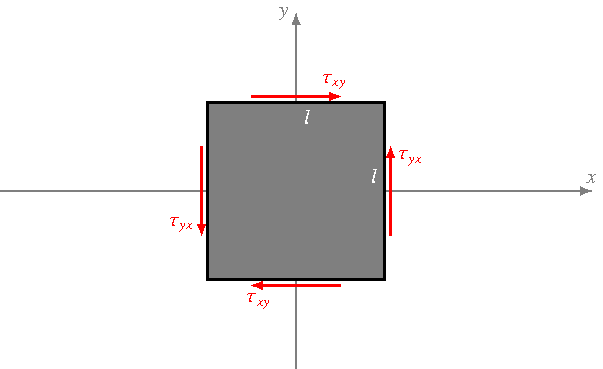
\includegraphics{chapters/2/drehmoment.pdf}
\caption{Drehmoment um die $z$-Achse der Schwerkräfte auf einen Würfel
mit Kantenlänge $2l$. Gezeigt sind nur die Komponenten von $\bm{\tau}$,
die zu einem Drehmoment führen.
\label{skript:drehmoment}}
\end{figure}
In diesem Abschnitt wollen wir nachweisen, dass der Spannungstensor
symmetrisch ist.
Dazu betrachten wir das Drehmoment, welches die Scherkräfte auf einen
kleinen Würfel mit Kantenlänge $2l$ ausüben (Abbildung \ref{skript:drehmoment}).

Der Würfel hat die Masse $m=\varrho(2l)^3$.
Das Trägheitsmoment eines Würfels mit Masse $m$ und Kantenlänge $2l$
ist
\[
I_z
=
\frac1{12}m((2l)^2+(2l)^2)
=
\frac1{12}\varrho 8l^3\cdot8l^2
=
\frac{16}{3}\varrho l^5.
\]
Der Drehimpuls um die $z$-Achse ist $L_z=I_z\omega$.

Aus Abbildung~\ref{skript:drehmoment} kann man die Scherkräfte auf den
Seitenflächen ablesen, sie sind $\tau_{xy}4l^2$ bzw.~$\tau_{yx}4l^2$,
ihr Hebelarm ist $l$.
Das resultierende Drehmoment um die $z$-Achse ist daher
\[
M_z = 8l^3\tau_{xy} - 8l^3\tau_{yx}.
\]
Die Bewegungsgleichungen eines starren Körpers besagen jetzt, dass
für die Winkelgeschwindigkeit der Drehung des Würfels um die $z$-Achse
die Gleichung
\[
\frac{dL_z}{dt}
=
M_z
\qquad\Rightarrow\qquad
I_z\dot\omega
=
M_z
\qquad\Rightarrow\qquad
\dot\omega
=
\frac{M_z}{I_z}
=
\frac{8l^3(\tau_{xy}-\tau_{yx})}{\frac{16}{3}l^5}
=
\frac{3}{2l^2}(\tau_{xy}-\tau_{yx}).
\]
Wir nehmen an, es sei $\tau_{xy}\ne\tau_{yx}$.
Lässt man $l$ gegen $0$ gehen, folgt die Aussage, dass die
Winkelgeschwindigkeit eines sehr kleinen Würfels im Fluid sich mit beliebig
schnell anwachsender Winkelgeschwindigkeit drehen müsste.
Dieses unphysikalische Resultat erlaubt zu schliessen, dass
$\tau_{xy}=\tau_{yx}$ sein muss und dass nur ein
symmetrischer Spannungstensor ein physikalisches Fluid beschreibt.

\subsubsection{Druck und Spannungen}
Die Diagonalelemente des Spannungstensors $\bm{\tau}$ beschreiben
Normalkräfte auf ein Volumenelement des Fluids.
Im Gleichgewicht sind sie alle gleich gross und stimmen mit dem
negativen {\em (hydrostatischen) Druck} überein, wir setzen daher
\index{Druck}
\index{hydrostatischer Druck}
\[
p=-\frac13\operatorname{Spur}\bm{\tau}.
\]
Wir können daher $\bm{\tau}$ zerlegen in eine Diagonalmatrix
mit Elementen $-p$ auf der Diagonalen und eine spurlose Matrix
\[
\bm{\tau} = -pE + \bm{\sigma},
\]
$E$ ist die Einheitsmatrix.
Die spurlose symmetrische Matrix $\bm{\sigma}$ heisst auch
{\em Spannungsdeviator}.
\index{Spannungsdeviator}

Für die Bewegungsgleichung brauchen wir die Divergenz beider Terme.
Die Druckterme sind alle gleich, nach
Definition~\ref{skript:definition divergenz} ist
\[
(\nabla\cdot(pE))_x
=
\sum_i
\frac{\partial p\delta_{xi}}{\partial i}
=
\frac{\partial p}{\partial x}
\qquad\Rightarrow\qquad
\nabla\cdot(pE)
=
\nabla p.
\]
Damit wird die Bewegungsgleichung 
\begin{equation}
\frac{\partial \varrho\vec{v}}{\partial t}
=
-\nabla\cdot(\varrho\vec{v}\vec{v})
+\varrho\vec b
-\nabla p
+\nabla\cdot\bm{\sigma}
\label{skript:navier-stokes2}
\end{equation}
Die Scherkräfte sind in einem newtonschen Fluid proportional zu
den Schergeschwindigkeiten.
Man kann zeigen (siehe \cite[p.~172]{skript:kaperengler}), dass $\bm{\sigma}$
geschrieben werden kann als
\[
\bm{\sigma}
=
2\nu\biggl(\bm{\varepsilon} - \frac13(\nabla\cdot\vec{v})E\biggr)
\qquad\text{mit}\qquad
\bm{\varepsilon}=\frac12\bigl(\nabla\vec{v}+(\nabla\vec{v})^t\bigr).
\]
Die spezielle Form von $\bm{\varepsilon}$ ist notwendig, damit die Matrix
$\bm{\varepsilon}$ symmetrisch wird.
Der zweite Term im Ausdruck von $\bm{\sigma}$ ist nötig, damit die Spur
\[
\operatorname{Spur}{\bm{\sigma}}
=
2\nu(\operatorname{\varepsilon} - \nabla\cdot\vec{v})
=
2\nu
\frac12
\biggl(
\sum_i \frac{\partial v_i}{\partial i}
+
\frac12
\sum_i \frac{\partial v_i}{\partial i}
-
\nabla\cdot\vec{v}
\biggr)
=
0
\]
von $\bm{\sigma}$ verschwindet.

Die Divergenz $\nabla\cdot\bm{\sigma}$ von $\bm{\sigma}$ kann damit explizit
durch die Geschwindigkeit ausgedrückt werden.
Wir berechnen die Divergenz der einzelnen Terme:
\begin{align}
(\nabla\cdot\bm{\varepsilon})_x
&=
\sum_i\frac{\partial \varepsilon_{ix}}{\partial i}
=
\frac12
\sum_i\frac{\partial}{\partial i}\biggl(
\frac{\partial v_i}{\partial x}+\frac{\partial v_x}{\partial i}
\biggr)
=
\frac{\partial}{\partial x}
\sum_i\frac{\partial v_i}{\partial i}
+
\frac12
\sum_i \frac{\partial^2 v_x}{\partial i^2}
=
\frac12\frac{\partial}{\partial x}
(\nabla\cdot\vec{v})
+
\frac12\Delta v_x
\notag
\\
\nabla\cdot\bm{\varepsilon}
&=
\frac12\nabla(\nabla\cdot\vec{v})
+
\frac12\Delta\vec{v}
\notag
\\
(\nabla\cdot(\nabla\cdot\vec{v})E)_x
&=
\sum_i \frac{\partial}{\partial i} (\nabla\cdot\vec{v}E)_{xi}
=
\sum_i \frac{\partial}{\partial i} (\nabla\cdot\vec{v}\delta_{xi})
=
\frac{\partial}{\partial x}(\nabla\cdot\vec{v})
\notag
\\
\nabla\cdot(\nabla\cdot\vec{v})E)
&=
\nabla(\nabla\cdot\vec v)
\notag
\\
\intertext{und erhalten so für die Divergenz von $\bm{\sigma}$:}
\nabla\cdot\bm{\sigma}
&=
2\nu\biggl(
\nabla\cdot\bm{\varepsilon}
-\frac13\nabla\cdot((\nabla\cdot\vec{v})E)
\biggr)
=
2\nu\biggl(
\frac12
\nabla(\nabla\cdot\vec{v})
+
\frac12\Delta\vec{v}
-\frac13
\nabla(\nabla\cdot\vec{v})
\biggr)
\\
&=
\nu\Delta\vec{v}
+\frac{\nu}3\nabla(\nabla\cdot\vec{v}).
\label{skript:sigmadiv}
\end{align}

\subsubsection{Inkompressible Strömung}
In einem inkompressiblen Fluid ist $\nabla\cdot\vec{v}=0$, dann fällt
der zweite Term in \eqref{skript:sigmadiv} weg.
Die Strömungsgleichung eines inkompressiblen Fluids erhält damit die
einfache Form
\begin{equation}
\frac{\partial\vec{v}}{\partial t}
=
-\nabla\cdot(\vec{v}\vec{v})
+\vec{b}
-\frac1{\varrho}(\nabla p
-\nu\Delta\vec{v}),
\label{skript:inkompressibel newtonsch}
\end{equation}
die klassische Navier-Stokes Gleichung.

\subsection{Zustandsgleichungen}
Die Dichte hängt vor allem auch von der Temperatur ab.
In den Ozeanen ändert die Dichte des Wassers mit dem Salzgehalt.
Eine vollständige Beschreibung der Strömung in Ozeanen oder der
Atmosphäre muss daher auch noch weitere Variablen modellieren.
In Kapitel~\ref{chapter:wetter und klima} haben wir bereits auf die
Wärmeleitungsgleichungen hingewiesen.

Die Felder $T$, $p$ und $\varrho$ sind bei einem idealen Gas miteinander
durch die Zustandsgleichung
\[
p=\varrho T R_s
\]
mit der spezifischen Gaskonstante $R_s$ verbunden.
Für den Zusammenhang von Dichte, Temperatur und Salzgehalt gibt
es jedoch kein derart einfaches Modell.
Eine weitere Kopplung zwischen der Temperatur und der
Strömung entsteht durch die Viskosität $\nu$, die sehr stark
von der Temperatur abhängt.
Auch dafür gibt es keine einfachen Modell.

In vielen Fällen schwanken die physikalischen Grössen nur geringfügig
um einen Mittelwert.
Zum Beispiel hängt die Dichte $\varrho$ von Meerwasser sowohl von
der Temperatur $T$ als auch vom Salzgehalt $h$ ab, die Dichte ist
also eine Funktion $\varrho(T,h)$.
Wir können $\varrho$ als Taylorreihe um die mittlere Temperatur $T_0$
und den mittleren Salzgehalt $h_0$ entwickeln:
\[
\varrho(T,h)
=
\varrho_0 -\alpha(T-T_0) + \beta(h-h_0).
\]
In Klimamodellen betrachten wir typischerweise nur kleine Abweichungen
von Mittelwerten, so dass ein solches Modell sehr erfolgreich sein kann.

\subsection{Boussinesq-Approximation}
Die Strömung in der Erdatmosphäre kann offensichtlich nicht als
inkompressibel betrachtet werden, die Dichte ist offenbar nicht
konstant.
Der Zustand der Atmosphäre weicht jedoch nur wenig einem mittleren
Dichteprofil $\varrho_0$ ab, welches im wesentlich durch das Temperaturprofil
festgelegt ist.
Im Normalzustand nimmt die Temperatur der Atmosphäre ziemlich genau
linear ab bis zur Höhe der Thermopause.
Auf die horizontale Komponente der Strömung hat eine Abweichung des
Temperaturprofils kaum einen Einfluss, denn andere Terme der
Navier-Stokes-Gleichung
\eqref{skript:navier-stokes2}
sind bedeutender.
Für die vertikale Bewegung ist der Term der äusseren Kräfte,
nämlich die Schwerkraft, dominant.
Wir können dies berücksichtigen, indem wir die Erdbeschleunigung
$g$ durch
\begin{equation}
g\frac{\varrho}{\varrho_0}
\label{skript:boussinesq}
\end{equation}
ersetzen.
Diese Approximation ist bekannt als die Boussinesq-Approximation.
Für unsere Zwecke hier brauchen wir nicht mehr als \eqref{skript:boussinesq}.
Dies wird bei der Herleitung der Lorenz-Gleichung in Abschnitt
\ref{section:lorenz-modell} benötigt.
Für die vollständigen Boussinesq-Gleichungen siehe \cite{skript:kaperengler}.

%In der Navier-Stokes-Gleichung können wir die horizontale Bewegung
%von der vertikalen vollständig trennen.
%Wir schreiben dazu
%\[
%\vec{u}
%=
%\begin{pmatrix}v_x\\v_y\end{pmatrix},
%\qquad
%w=v_z.
%\]
%Ausser in den für den Auftrieb wesentlichen Termen (Druck und äussere Kräfte)
%betrachten wir die Dichte als konstant.
%Die Kontinuitätsgleichung wird daher zu
%\[
%\nabla\cdot\vec{u}\frac{\partial w}{\partial z} = 0.
%\]
%Dies besagt, dass die Quellen des horizontalen Strömungsfeldes 
%durch die Vertikalströmung gespeist werden.
%Die horizontale Bewegungsgleichung bleibt bis auf den Druckterm
%erhalten.

\subsection{Inkompressible zweidimensionale Strömung}
Die Kontinuitätsgleichung
und die Navier-Stokes-Gleichung gelten auch für eine zweidimensionale
Strömung.
Im Allgmeinen ist die Strömung nicht wesentlich leichter zu berechnen.
Nur im Falle einer inkompressiblen Strömung oder der Boussinesq-Approximation
spielt die Dichte in den Gleichungen keine Rolle, was erlaubt,
sie weiter zu vereinfachen:
\begin{align}
0
&=
-\nabla\cdot\vec v
\label{skript:2dim kontinuitaet}
\\
\frac{\partial \vec{v}}{\partial t}
&=
-\nabla\cdot(\vec{v}\vec{v})+\vec b + \frac1{\varrho}\nabla\cdot\bm{\tau}.
\label{skript:2dim navier-stokes}
\end{align}
Im Falle der Boussinesq-Approximation kommt auf der rechten Seite noch
ein Term für die Auftriebskraft hinzu.

Die Gleichungen
\eqref{skript:2dim kontinuitaet}
und
\eqref{skript:2dim navier-stokes}
bilden ein System von partiellen Differentialgleichungen für die zwei
unbekannten Funktionen $v_x$ und $v_y$, die Komponenten der 
Strömungsgeschwindigkeit.
Wir werden im Folgenden zeigen, dass die 
\eqref{skript:2dim kontinuitaet}
ermöglicht, das System auf eine einzelne partielle Differentialgleichung
für nur eine einzige Funktion zu reduzieren.

\subsubsection{Satz von Green}
\begin{figure}
\centering
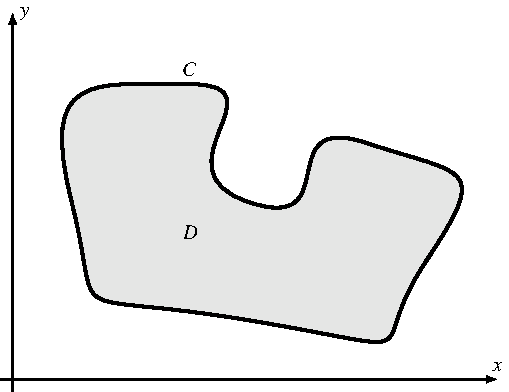
\includegraphics{chapters/2/green-curve.pdf}
\caption{Satz von Green: Das Wegintegral entlang der Randkurve $C$
stimmt mit dem zweifachen Integral über $D$ überein.
\label{skript:green-kurve}}
\end{figure}
Die Kontinuitätsgleichung 
\eqref{skript:2dim kontinuitaet}
ist ausgeschrieben
\[
0
=
\nabla\cdot\vec v
=
\frac{\partial v_x}{\partial x} + \frac{\partial v_y}{\partial y}.
\]
Die Divergenz auf der rechten Seite kommt auch im Satz von Green
vor:

\begin{satz}[Green]
\label{skript:2dim green}
Sei $D$ in kompaktes Gebiet in der $x$-$y$-Ebene mit Rand $\partial D=C$.
Weiter seien $f,g\colon D\to\mathbb R$ stetige Funktionen, die in $D$ 
stetig differenzierbar sind.
Dann gilt
\begin{equation}
\iint_{D}
\frac{\partial g(x,y)}{\partial x}
-
\frac{\partial f(x,y)}{\partial y}\,dx\,dy
=
\oint_C (f(x,y)\,dx + g(x,y)\,dy)
\label{skript:green formel}
\end{equation}
(Abbildung~\ref{skript:green-kurve}).
\end{satz}

Das Integral auf der rechten Seite wird mit Hilfe einer Parametrisierung
$\gamma\colon [a,b]\to\mathbb R^2$ der Randkurve $C$ definiert.
\begin{align*}
\oint_C f(x,y)\,dx
&=
\int_a^b f(\gamma_x(t),\gamma_y(t))\dot{\gamma}_x(t)\,dt,
\\
\oint_C g(x,y)\,dy
&=
\int_a^b g(\gamma_x(t),\gamma_y(t))\dot{\gamma}_y(t)\,dt.
\end{align*}
Es kann auch vektoriell mit dem Skalarprodukt als
\[
\oint_C
\underbrace{
\begin{pmatrix}f\\g\end{pmatrix}
}_{\displaystyle =\vec{w}}
\cdot
\begin{pmatrix}\dot\gamma_x\\\dot\gamma_y\end{pmatrix}
\,dt
=
\oint_C \vec{w}\cdot\dot\gamma(t)\,dt
=:
\oint_C \vec{w}\cdot d\vec{s}
\]
geschrieben werden kann.

\subsubsection{Stromfunktion}
Wir wenden den Satz \ref{skript:2dim green} von Green auf die
Funktionen $f(x,y)=-v_y(x,y)$ und $g(x,y)=v_x(x,y)$ an.
Die Formel \eqref{skript:green formel} ergibt
\begin{equation}
\oint_C (-v_y(x,y)\,dx + v_x(x,y)\,dy)
=
\iint_D
\underbrace{
\frac{\partial v_x(x,y)}{\partial x}
+
\frac{\partial v_y(x,y)}{\partial y}
}_{\displaystyle=0}
\,dx\,dy
=
0.
\label{skript:wegunabh}
\end{equation}
Man kann dieses Resultat auch wie folgt interpretieren.
Wenn $C_1$ und $C_2$ zwei Kurven sind, die den Punkt $A$ mit dem Punkt $B$
verbinden, dann lässt sich eine geschlossene Kurve $C$ konstruieren, indem
zuerst die Kurve $C_1$ von $A$ nach $B$ durchlaufen wird und dann die
Kurve $C_2$ in umgekehrter Richtung von $B$ nach $A$.
Die Formel \eqref{skript:wegunabh} besagt dann, dass 
\begin{align*}
0
&=
\oint_{C} (-v_y(x,y)\,dx + v_x(x,y)\,dy)
\\
&=
\int_{C_1} (-v_y(x,y)\,dx + v_x(x,y)\,dy)
-
\int_{C_2} (-v_y(x,y)\,dx + v_x(x,y)\,dy)
\end{align*}
oder
\begin{align*}
\Rightarrow
\qquad
\int_{C_1} (-v_y(x,y)\,dx + v_x(x,y)\,dy)
&=
\int_{C_2} (-v_y(x,y)\,dx + v_x(x,y)\,dy).
\end{align*}
Das Wegintegral hängt also nicht von der Wahl des Weges ab, jeder Weg
von $A$ nach $B$ führt auf den gleichen Wert des Integrals.

\begin{figure}
\centering
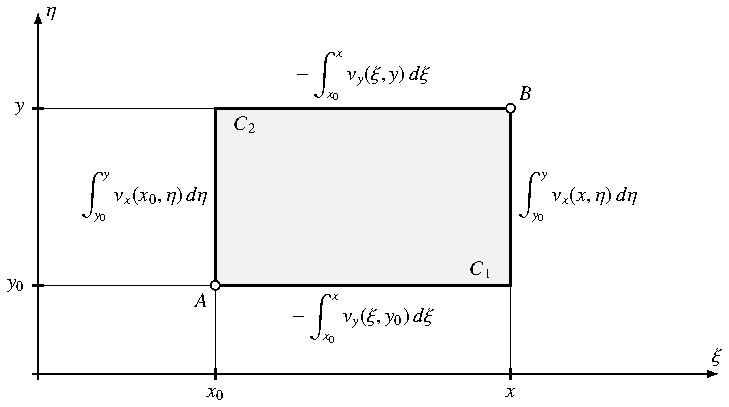
\includegraphics{chapters/2/green-curves.pdf}
\caption{Verschiedene Pfade zur Berechnung der Funktion $\psi(B)$
führen auf den gleichen Wert von $\psi(B)$ und ermöglichen, die partiellen
Ableitungen zu berechnent.
\label{skript:psi-pfade}}
\end{figure}

Wir halten den Punkt $A$ fest und definieren die Funktion
\[
\psi(B)
=
\int_C (-v_y(x,y)\,dx + v_x(x,y)\,dy)
\]
für einen beliebigen Weg von $A$ nach $B$. 
Zum Beispiel können für die Berechnung die Kurven
$C_1$ oder $C_2$ in Abbildung~\ref{skript:psi-pfade}
verwendet werden.
Damit lassen sich die Integrale ausschreiben:
\begin{align*}
\psi(x,y)
&=
\int_{C_1} (-v_y(x,y)\,dx + v_x(x,y)\,dy)
=
-\int_{x_0}^x v_y(\xi, y_0)\,d\xi
+
\int_{y_0}^y v_x(x,\eta)\,d\eta
\\
&=
\int_{C_2} (-v_y(x,y)\,dx + v_x(x,y)\,dy)
=
\int_{y_0}^y v_x(x_0,\eta)\,d\eta
-
\int_{x_0}^x v_y(\xi,y)\,d\xi.
\end{align*}
Diese Ausdrücke erlauben uns, die partiellen Ableitungen von $\psi(x,y)$
zu berechnen.
Für die Ableitung nach $x$ verwenden wir den zweiten Ausdruck, für die
Ableitung nach $y$ den ersten.
Wir erhalten
\begin{align*}
\frac{\partial\psi(x,y)}{\partial x}
&=
-\frac{\partial}{\partial x} \int_{x_0}^x v_y(\xi,y)\,d\xi
=
-v_y(x,y),
\\
\frac{\partial\psi(x,y)}{\partial y}
&=
\frac{\partial}{\partial y} \int_{y_0}^y v_x(x,\eta)\,d\eta
=
v_x(x,y).
\end{align*}
In vektorieller Form kann man dies auch als
\begin{equation}
\vec{v}
=
\begin{pmatrix}v_x\\v_y \end{pmatrix}
=
\underbrace{
\begin{pmatrix}0&-1\\1&0\end{pmatrix}
}_{\displaystyle=J}
\begin{pmatrix}
\frac{\partial\psi}{\partial x}\\
\frac{\partial\psi}{\partial y}
\end{pmatrix}
=
J\nabla\psi
\label{skript:Jnablapsi}
\end{equation}
schreiben.
Aus der Funktion $\psi$ lässt sich das Vektorfeld $\vec{v}$ also wieder
rekonstruieren.
Sie heisst die {\em Stromfunktion} des Vektorfeldes $\vec{v}$.
\index{Stromfunktion}
Natürlich ist $\psi(x,y)$ nur bis auf eine Konstante bestimmt.

Umgekehrt ist für jede beliebige Funktion $\varphi(x,y)$ das Vektorfeld
$\vec{u}=J\nabla\varphi$ divergenzfrei:
\begin{align*}
\nabla\cdot\vec{u}
=
\frac{\partial}{\partial x}
\biggl(-\frac{\partial\varphi}{\partial y}\biggr)
+
\frac{\partial}{\partial y}
\biggl(\frac{\partial\varphi}{\partial x}\biggr)
=
-\frac{\partial^2\varphi}{\partial x\,\partial y}
+\frac{\partial^2\varphi}{\partial y\,\partial x}
=
0.
\end{align*}
Die Darstellung \eqref{skript:Jnablapsi} des Geschwindigkeitsfeldes 
erlaubt eine geometrische Interpretation.
Der Gradient $\nabla\psi$ ist ein Vektorfeld, welches auf den
Niveaulinien der Funktion $\psi$ senkrecht steht.
Je schneller die Zunahme von $\psi$, desto grösser ist der
Vektor $\nabla\psi$.

Die Matrix $J$ ist eine Drehmatrix, sie dreht Vektoren um $90^\circ$ 
im Gegenuhrzeigersinn.
Die Vektoren $J\nabla\psi$ sind also tangential an die Niveaulinien,
die Niveaulinien sind also gleichzeitig die Stromlinien der Strömung.
Ist die Strömung auf ein kompaktes Gebiet beschränkt, dann ist der
Rand des Gebietes eine Stromlinie, also eine Niveaulinie von $\psi$.
Da $\psi$ nur bis auf eine Konstante festgelegt ist, kann man $\psi$
so wählen, dass der Rand des Gebietes durch die Gleichung $\psi(x,y)=0$
beschrieben wird.

\index{Stromlinien}
\begin{figure}
\centering
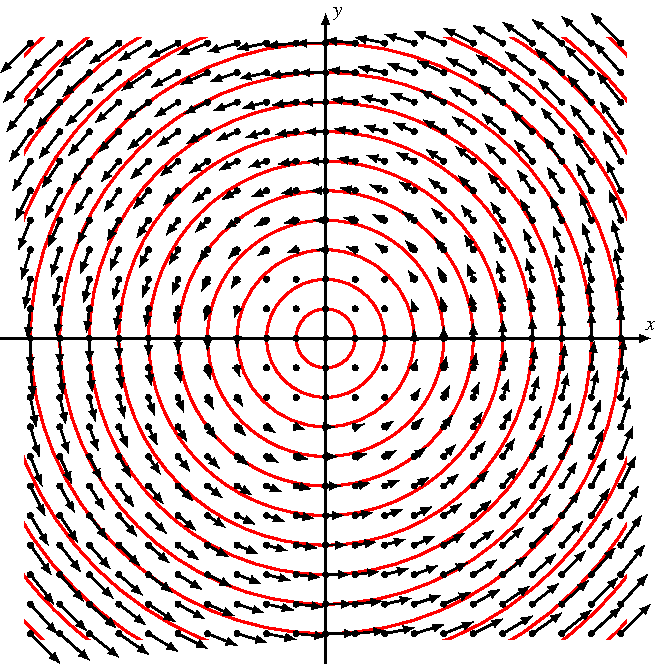
\includegraphics{chapters/2/rotation.pdf}
\caption{Strömungsfunktion $\psi(x,y)=a(x^2+y^2)$ und das zugehörige
Vektorfeld.
Die Strömungsgeschwindigkeit ist proportional zum Radius, es handelt
sich also um eine starre Drehung um den Nullpunkt.
\label{skript:rotation}}
\end{figure}
Die Funktion $\psi(x,y)=a(x^2+y^2)$ führt auf das Vektorfeld
\[
\vec{v}
=
J\nabla\psi
=
2a
\begin{pmatrix}
-y\\x
\end{pmatrix}
\]
(Abbildung~\ref{skript:rotation}).
Die Strömungsgeschwindigkeit ist $2a\sqrt{x^2+y^2}=2ar$, es handelt sich
also um eine starre Drehung um den Nullpunkt des Koordinatensystems mit
Winkelgeschwindigkeit $\omega=2a$.

\subsubsection{Vorticity}
Wir suchen eine Grösse, mit der wir das Ausmass messen können, wie schnell
sich das Fluid dreht.
Die Winkelgeschwindigkeit bei der Drehung um den Punkt $(x,y)$ können wir
durch Vergleich der Geschwindigkeit an den Punkten $(x\pm h,y)$ und
$(x,y\pm h)$ finden.
Es ist
\[
\omega
=
\frac{v_y(x+h),y) - v_y(x-h,y)}{2h}
=
\frac{-v_x(x,y+h) + v_x(x,y-h)}{2h}.
\]
Beim Grenzübergang $h\to 0$ erhalten wir
\[
\omega
=
\frac{\partial v_y(x,y)}{\partial x}
=
-\frac{\partial v_x{x,y}}{\partial y}
\qquad\text{oder}\qquad
2\omega
=
\frac{\partial v_y}{\partial x}-\frac{\partial v_x}{\partial y}.
\]
Damit haben wir eine Grösse gefunden, die als Mass für die Drehgeschwindigkeit
dienen kann.
\index{Vorticity}
\begin{definition}
Ist $\vec{v}$ das Geschwindigkeitsfeld der Strömung, dann schreiben wir
\[
\nabla\times\vec{v}
=
\frac{\partial v_y}{\partial x}-\frac{\partial v_x}{\partial y}
=
\zeta.
\]
Die Funktion $\zeta$ heisst die {\em Vorticity} des Strömungsfeldes.
\end{definition}

Beschreibt man die Strömung mit Hilfe der Strömungsfunktion, dann gilt
für die Vorticity
\begin{equation}
\zeta
=
\nabla\times\vec{v}
=
\nabla\times J\nabla\psi
=
\frac{\partial}{\partial x}
\biggl(-\frac{\partial\psi}{\partial y}\biggr)
-
\frac{\partial}{\partial x}
\frac{\partial\psi}{\partial x}
=
-\biggl(
\frac{\partial^2\psi}{\partial x^2}
+
\frac{\partial^2\psi}{\partial y^2}
\biggr)
=
-\Delta \psi.
\label{skript:stroemung-vorticity}
\end{equation}
Der Laplace-Operator verbindet also die Strömungsfunktion direkt mit der
Vorticity.
Für die Strömung in einem kompakten Gebiet $\Omega$ ist der Rand eine
Niveaulinie von $\psi$.
Wie früher dargelegt können wir $\psi$ so wählen, dass $\psi=0$ gilt auf
dem Rand.
Bei gegebener Vorticity $\zeta$ ist daher $\psi$ die Lösung der
partiellen Differentialgleichung
\begin{equation}
\Delta \psi = -\zeta\quad\text{in $\Omega$}
\qquad
\psi = 0\quad\text{auf $\partial\Omega$}.
\label{skript:zetapsielliptisch}
\end{equation}
Die Theorie der elliptischen partiellen Differentialgleichungen 
sagt, dass $\psi$ eindeutig bestimmt ist.
Statt die Strömungsgleichungen für $\psi$ zu lösen, können wir
also auch versuchen, eine Gleichung für die Vorticity $\zeta$
aufzustellen und dann mit Hilfe des elliptischen partiellen
Randwertproblems \eqref{skript:zetapsielliptisch} die Strömungsfunktion
und schliesslich $\vec{v}$ bestimmen.

Um die Differentialgleichung für $\zeta$ zu finden, wenden wir den
Operator $\nabla\times\mathstrut$ auf die Bewegungsgleichung
\eqref{skript:2dim navier-stokes}
an:
\[
\nabla\times\frac{\partial \vec{v}}{\partial t}
=
-\nabla\times(\nabla\cdot(\vec{v}\vec{v}))+\nabla\times\vec b + \nabla\times\biggl(\frac1{\varrho}\nabla\cdot\bm{\tau}\biggr).
\]
Die linke Seite ist die Zeitableitung der Vorticity.
Die Divergenz von $\vec{v}\vec{v}$ ist 
\[
(\nabla\cdot(\vec{v}\vec{v}))_j
=
\sum_i \frac{\partial}{\partial i}v_iv_j
=
\biggl(\sum_i \frac{\partial v_i}{\partial i}\biggr)v_j
+
\sum_i v_i\frac{\partial v_j}{\partial i}
=
(\underbrace{\nabla\cdot\vec{v}}_{\displaystyle=0})v_j
+
\vec{v}\cdot\nabla v_j.
\]
Es folgt
\[
\nabla\cdot(\vec{v}\vec{v})
=
\vec{v}\cdot\nabla \vec{v}.
\]
Daraus kann man jetzt auch die Vorticity berechnen:
\begin{align*}
\nabla\times(\nabla\cdot(\vec{v}\vec{v}))
&=
\nabla\times(\vec{v}\cdot\nabla\vec{v})
=
\frac{\partial}{\partial x}(\vec{v}\cdot\nabla v_y)
-
\frac{\partial}{\partial y}(\vec{v}\cdot\nabla v_x)
\\
&=
\vec{v}\cdot\nabla
\biggl(\frac{\partial v_y}{\partial x}-\frac{\partial v_x}{\partial y}\biggr)
+
\frac{\partial\vec{v}}{\partial x} \cdot\nabla v_y
-
\frac{\partial\vec{v}}{\partial y} \cdot\nabla v_x
\\
&=
\vec{v}\cdot\nabla\zeta
+
\frac{\partial v_x}{\partial x} \frac{\partial v_y}{\partial x}
+
\frac{\partial v_y}{\partial x} \frac{\partial v_y}{\partial y}
-
\frac{\partial v_x}{\partial y} \frac{\partial v_x}{\partial x}
-
\frac{\partial v_y}{\partial y} \frac{\partial v_x}{\partial y}
\\
&=
\vec{v}\cdot\nabla\zeta
+
\frac{\partial v_x}{\partial x}
\biggl(\frac{\partial v_y}{\partial x}-\frac{\partial v_x}{\partial y}\biggr)
+
\frac{\partial v_y}{\partial y}
\biggl(\frac{\partial v_y}{\partial x}-\frac{\partial v_x}{\partial y}\biggr)
\\
&=
\vec{v}\cdot\nabla\zeta
+
(\nabla\cdot\vec{v})\zeta
=
\vec{v}\cdot\nabla\zeta.
\end{align*}
Wir waren also nicht ganz erfolgreich, die Geschwindigkeit aus der
Bewegungsgleichung zu eliminieren.
Wir haben nur die Form
\[
\frac{\partial \zeta}{\partial t}
=
-\vec{v}\cdot\nabla\zeta
+\nabla\times\vec b
+ \nabla\times\biggl(\frac1{\varrho}\nabla\cdot\bm{\tau}\biggr)
\]
erreicht.
Ausserdem ist es möglich, dass die Spannungen $\bm{\tau}$ ebenfalls von
den Geschwindigkeiten abhängig sind.

Wir können aber die Vorticity auch noch durch die Strömungsfunktion
ausdrücken.
Ersetzen wir $\zeta=-\Delta\psi$ in der Bewegungsgleichung, erhalten
wir
\begin{equation}
\frac{\partial \Delta \psi}{\partial t}
=
-J\nabla\psi\cdot\nabla\Delta\psi
+\nabla\times\vec b
+ \nabla\times\biggl(\frac1{\varrho}\nabla\cdot\bm{\tau}\biggr).
\label{skript:voritictyequation}
\end{equation}
Jetzt ist die Strömung vollständig durch die einzige unbekannte Funktion 
$\psi$.

Der erste Term auf der rechten Seite von \eqref{skript:voritictyequation}
kann noch etwas kompakter geschrieben werden.
Es ist
\begin{align*}
(J\nabla f)\cdot(\nabla g)
&=
\begin{pmatrix}
-\frac{\partial f}{\partial y}
\\
\frac{\partial f}{\partial x}
\end{pmatrix}
\cdot
\begin{pmatrix}
\frac{\partial g}{\partial x}\\
\frac{\partial g}{\partial y}
\end{pmatrix}
=
\frac{\partial f}{\partial x}
\frac{\partial g}{\partial y}
-\frac{\partial f}{\partial y}
\frac{\partial g}{\partial x}.
\end{align*}
Der Ausdruck auf der rechten Seite kommt auch in anderem Zusammenhang vor.

\begin{definition}
Seien $f$ und $g$ Funktionen der Variablen $x$ und $y$.
Dann heisst
\[
\frac{\partial(f,g)}{\partial(x,y)}
=
\frac{\partial f}{\partial x}
\frac{\partial g}{\partial y}
-
\frac{\partial f}{\partial y}
\frac{\partial g}{\partial x}
\]
die
{\em Funktionaldeterminante} oder {\em Jacobische Determinante} von
$f$ und $g$.
\end{definition}
\index{Funktionaldeterminante}
\index{Jacobi-Determinante}
Mit dieser Definition wird die Bewegungsgleichung
\begin{equation}
\frac{\partial \Delta \psi}{\partial t}
=
\nabla\times\vec b
+ \nabla\times\biggl(\frac1{\varrho}\nabla\cdot\bm{\tau}\biggr)
-\frac{\partial(\psi,\Delta\psi)}{\partial(x,y)}.
\label{skript:psidgl}
\end{equation}
Im Falle der Boussinesq-Näherung kommt noch ein Term für den
Auftrieb hinzu.

\subsubsection{Spannungen und Stromfunktion}
Für eine newtonsche Flüssigkeit haben wir in 
\eqref{skript:inkompressibel newtonsch}
bereits den Spannungstensor durch den Druck und die Spannungen
ausgedrückt.
Aus der Bewegungsgleichung für die Geschwindigkeit haben wir die
Differentialgleichung \eqref{skript:psidgl} erhalten, indem
wir den Operator $\nabla\times\mathstrut$ angewendet haben.
Wir müssen jetzt also 
\[
\nabla\times\biggl(\frac1{\varrho}(\nabla p-\nu\Delta\vec{v})\biggr)
=
\frac{1}{\varrho}
\biggl(
\nabla\times\nabla p
-
\nu \nabla\times\Delta\vec{v}
\biggr)
=
\frac1{\varrho}
\biggl(
\frac{\partial}{\partial x}\frac{\partial p}{\partial y}
-
\frac{\partial}{\partial y}\frac{\partial p}{\partial x}
-\nu\Delta\nabla\times\vec{v}
\biggr)
\]
berechnen.
Der erste Term fällt weg, weil es auf die Reihenfolge der zweiten
Ableitungen nicht ankommt.
Im zweiten Term haben wir angenommen, dass $\nu$ nicht vom Ort
abhängig.
Dies ist genau genommen nicht richtig, da $\nu$ zum Beispiel
stark von der Temperatur abhängt, die ebenfalls nicht konstant sein
muss.
Der zweite Term in der Klammer ist natürlich einfach
$\nu\Delta\zeta=-\nu\Delta^2\psi$.
Damit bekommen wir die Bewegungsgleichung für $\psi$ in der Form
\begin{equation}
\frac{\partial \Delta \psi}{\partial t}
=
\nabla\times\vec b
+\frac{\nu}{\varrho}\Delta^2\psi
-\frac{\partial(\psi,\Delta\psi)}{\partial(x,y)}.
\label{skript:psidgl2}
\end{equation}



%
% lorenz.tex -- Lorenz-Modell
%
% - Herleitung aus den Gleichungen der Fluiddynamik
% - Dynamik aus numerischen Simulationen
%
% (c) 2018 Prof Dr Andreas Müller, Hochschule Rapperswil
%
\section{Lorenz-Modell\label{section:lorenz-modell}}
Sowohl die Atmosphäre als auch die Ozeane werden durch die hydrodynamischen
Gleichungen beschrieben.
Es stellt sich damit die Frage, in welchem Masse sich daraus eine praktikable
Vorhersage sowohl von Wetter also auch des Klimas ableiten lässt.
In den Sechzigerjahren hat Edward Lorenz versucht, diese Frage mit einem
vereinfachten Modell zu beantworten.
Ziel dieses Abschnittes ist, das Lorenz-Modell aus den Gleichungen der
Fluiddynamik herzuleiten.

\subsection{Modellbeschreibung}
\begin{figure}
\centering
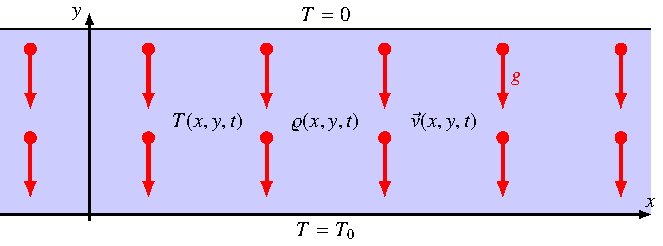
\includegraphics{chapters/2/lorenz-definition.pdf}
\caption{Definitionsgebiet für das Lorenz-Modell der Atmosphäre.
Gesucht sind Temperatur $T(x,y,t)$, Dichte $\varrho(x,y,t)$ und
Geschwindigkeit $\vec{v}(x,y,t)$ in einem Rechteckgebiet
$\mathbb R\times [0,\pi]$.
Die Temperatur ist an den Rändern vorgegeben, es gilt
$T(x,0,t)=T_0$ und $T(x,\pi,t)=0$.
Im Inneren Gebiet wird die Schwerkraft $g$ auf die Luft.
\label{skript:lorenzmodell definitionsgebiet}}
\end{figure}
Es soll ein dünner Schnitt durch die Atmosphäre modelliert werden.
Da Atmosphäre im Vergleich zur Krümmung der Erdoberfläche sehr dünn ist,
können wir sie als eben annehmen.
Wir verwenden die Koordinate $x$ parallel zur Erdoberfläche und $y$ als Höhe
(Abbildung~\ref{skript:lorenzmodell definitionsgebiet}).
Gesucht ist also die Temperatur $T(x,y,t)$ und die Dichte $\varrho(x,y,t)$
in Abhängigkeit von Position und Zeit sowie der Geschwindigkeitsvektor
\[
\vec v
=
\begin{pmatrix}v_x\\v_y\end{pmatrix}
=
\begin{pmatrix}v_x(x,y,t)\\v_y(x,y,t)\end{pmatrix}.
\]
Die Funktionen $T$, $\varrho$, $v_x$ und $v_y$ sind definiert in einem
Streifen.
Der Einfachheit halber wählen wir die Höhe des Streifens als $\pi$.
Wir können dies erreichen, indem wir die Längeneinheit geeignet wählen:
ist $h$ die ``Dicke'' der Atmosphäre\footnote{Die Konvektion in der Atmosphäre,
welche vom Lorenz-Modell vor allem beschrieben wird, findet im Wesentlichen
nur im untersten Teil der Atmosphäre, der sogenannten Troposphäre statt.
Die Troposphäre zeichnet sich aus durch mehr oder weniger lineare
Temperaturabnahme bis zur Höhe der sogenannten Tropopause in etwa
10km Höhe.
Wir können also die Höhe der Tropopause als $h$ verwenden.}, wählen wir
$h/\pi$ als Längeneinheit.
Das Definitionsgebiet für die Funktionen ist daher $R=\mathbb R\times [0,\pi]$.

Die Temperatur der Atmosphäre an der Erdoberfläche wird im wesentlichen von
der Temperatur des Bodens bestimmt, der von der einfallenden Strahlung
ergewärmt wird, es soll also $T(x,0,t)=T_0$ gelten.
Am oberen Rand des Schnittes schliesst die sehr dünne Hochatmosphäre an,
die im Wesentlichen in einem Strahlungsgleichgewicht mit der Umgebung steht.
Da wir die Dichte im wesentlichen als konstant ansehen wollen und damit
den Einfluss der Temperatur auf die Dichte nicht exakt modellieren wollen,
sind wir nicht gezwungen, eine bestimmte Temperaturskala zu verwenden.
Wir können daher willkürlich die Temperatur am oberen Rand als
$T(x,\pi,t)=0$ festlegen.

Auf das Medium im Streifen wirkt natürlich die Erdbeschleunigung,
die wir ebenfalls als konstant annehmen dürfen, da die Dicke der 
Atmosphäre im Vergleich zum Erdradius sehr klein ist.

\subsubsection{Stabile Atmosphäre}
\begin{figure}
\centering
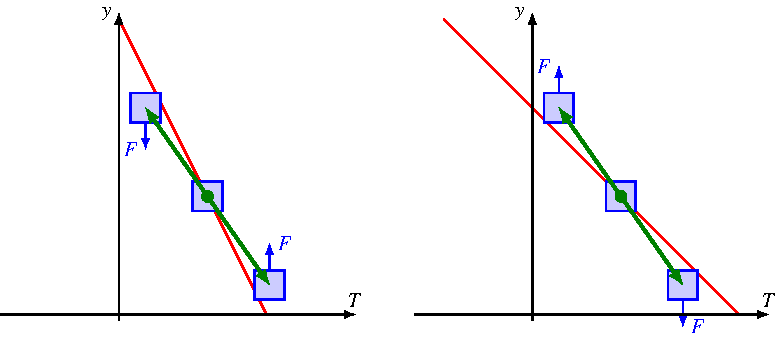
\includegraphics{chapters/2/lorenz-stabil.pdf}
\caption{Stabilität der Atmosphäre: bewegt sich ein Luftpaket in der
Atmosphäre nach oben oder unten, expandiert oder kontrahiert es und
verändert seine Temperatur adiabatisch (grün).
Ist diese Temperaturänderung grösser als der aktuelle Temperaturgradient
(links),
ändert sich die Dichte der Luft weniger stark als die der Umgebungsluft,
die Bewegung wird gestoppt, die Atmosphäre ist im Gleichgewicht.
Andernfalls wird die Bewegung beschleunigt, die Atmosphäre ist instabil
(rechts).
\label{skript:stabilitaet der atmosphaere}}
\end{figure}
Die Temperatur muss im Gebiet von unten nach oben abnehmen.
Aber auch der Druck muss mit zunehmender Höhe abnehmen. 
Wenn ein Luftpaket aufsteigt, wird es wegen des geringer werdenden
Druckes expandieren und damit adiabatisch abkühlen.
Wenn die Temperatur der umgebenden Luft schneller abnimmt als die
adiabatische Abkühlung, dann ist das Luftpaket in seiner neuen Höhe
wärmer und damit leichter als die Umgebung, es wird weiter ansteigen
(Abbildung~\ref{skript:stabilitaet der atmosphaere}).
Wenn die Temperatur der umgebenden Luft langsamer abnimmt als die
adiabatische Abkühlung, dann ist das Luftpaket in der neuen Höhe 
kälter und damit Dichter als die Umgebung, es wird wieder absinken.
Solange der Temperaturunterschied nicht zu gross ist, wird sich also ein
Zustand einstellen, in dem die Luft in Ruhe bleibt, der Wärmetransport
erfolgt ausschliesslich durch Wärmeleitung.

\subsubsection{Instabilität}
Bei genügend grosser Temperaturdifferenz wird die Atmosphäre jedoch
instabil, der Wärmetransport wird zusätzlich von Konvektion übernommen.
Die entstehenden Konvektionszellen können wegen der Translationssymmetrie
entlang der $x$-Achse an einer beliebigen Stelle entstehen, es gibt also
unendlich viele Lösungen, von denen eine gewählt werden muss.
In der Realität würden kleine Temperaturfluktionen dies unterstützen,
kleine Unterschiede in den Anfangsbedingungen führen also zu völlig
verschiedenen Strömungen.
% Abbildung?
Diese sensitive Abhängigkeit der Lösung von Anfangsbedingungen wird
oft als ein Kennzeichen von Chaos angesehen.

Im folgenden sollen zunächst die Gleichungen der Fluiddynamik auf die
vorliegende Situation spezialisiert werden.
Mit Hilfe eines geeigneten Ansatzes soll dann die partielle
Differentialgleichung weiter auf ein System von gewöhnlichen 
Differentialgleichungen reduziert werden.
In numerischen Simulationen soll schliesslich gezeigt werden, dass die 
Lorenz-Gleichungen tatsächlich chaotische Lösungen haben.

\subsubsection{Temperaturgleichung}
Wir haben in \eqref{skript:waermeleitungadvektion}
bereits eine Gleichung gefunden, welche den Wärmetransport in einem 
Fluid beschreibt.
Wir können daraus aber noch eine etwas einfacher zu handhabende Form
gewinnen, indem wir nur die Anomalie der Temperatur betrachten, also
die Abweichung vom Temperaturprofil, welches sich bei einem ruhenden
Fluid einstellt. 
Aufgrund der gewählten Geometrie ist 
\[
T_0(x,y,t)= T_0\biggl(1- \frac{y}{\pi}\biggr)
\]
in einem ruhenden Fluid, wir setzen daher
\[
\vartheta(x,y,t)
= 
T(x,y,t)
-
T_0\biggl(1-\frac{y}{\pi}\biggr)
\qquad\text{oder}\qquad
T(x,y,t)
=
T_0\biggl(1-\frac{y}{\pi}\biggr)
+
\vartheta(x,y,t)
\]
und setzen dies in die Gleichung \eqref{skript:waermeleitungadvektion}
ein.
Wir erhalten
\begin{align*}
\frac{\partial\vartheta}{\partial t}
&=
\frac{\partial T}{\partial t}
&
\Delta T
&=
\Delta \vartheta
\\
-\vec{v}\cdot\nabla T
&=
-\vec{v}\cdot\nabla\vartheta
+v_y\frac{T_0}{\pi}.
\\
\Rightarrow
\qquad
\frac{\partial\vartheta}{\partial t}
&=
-\vec{v}\cdot\nabla \vartheta
+v_y\frac{T_0}{\pi}
+
\kappa\Delta \vartheta.
\end{align*}
Die Geschwindigkeit kann mit Hilfe von $\vec{v}=-\nabla \psi$ wieder
durch die Stromfunktion ausgedrückt werden.
\begin{equation}
\frac{\partial\vartheta}{\partial t}
=
-J\nabla\psi\cdot\nabla\vartheta
+\frac{T_0}{\pi}\frac{\partial\psi}{\partial x}
+\kappa\Delta\vartheta
=
\kappa\Delta\vartheta
+\frac{T_0}{\pi}\frac{\partial\psi}{\partial x}
-\frac{\partial \psi}{\partial y}\frac{\partial \vartheta}{\partial x}
+\frac{\partial \psi}{\partial x}\frac{\partial \vartheta}{\partial y}
=
\kappa\Delta\vartheta
+\frac{T_0}{\pi}\frac{\partial\psi}{\partial x}
-
\frac{\partial(\psi,\vartheta)}{\partial(x,y)}.
\label{skript:lorenzthetagl}
\end{equation}
Man beachte, dass die Gleichung bis auf den ltzten Term linear 
in $\psi$ und $\vartheta$ ist.

\subsubsection{Bewegungsgleichung}
Die Bewegungsgleichung haben wir in
\eqref{skript:psidgl2}
bereits in die für ein zweidimensionales inkompressibles Fluid
geignete Form gebracht.
Da die Schwerkraft konstant ist, fällt der Terme $\nabla\times\vec{b}$
weg.

Aus der Boussinesq-Näherung
\eqref{skript:boussinesq}
erhalten wir noch einen Term, der den
Auftrieb beschreibt.
Auftrieb entsteht offenbar genau dann, wenn die Temperatur vom linearen
Temperaturprofil abweicht.
Wir nehmen an, dass die Dichteabweichung proportional zur Temperaturabweichung
ist, also
\[
\vec{b}
=
\begin{pmatrix}
0\\
-g(1-c\vartheta)
\end{pmatrix}
\qquad
\Rightarrow
\qquad
\nabla\times\vec{b}
=
c\frac{\partial\vartheta}{\partial x}.
\]
Damit erhalten wir die Bewegungsgleichung in der Form
\begin{equation}
\frac{\partial\Delta\psi}{\partial t}
=
\nu\Delta^2\psi 
+c\frac{\partial\vartheta}{\partial x}
-\frac{\partial(\psi,\Delta\psi)}{\partial(x,y)}.
\label{skript:lorenzpsigl}
\end{equation}
Man beachte, dass die Gleichung bis auf den letzten Term linear
in $\psi$ und $\vartheta$ ist.

\subsection{Grundgleichungen}
In den Gleichungen
\eqref{skript:lorenzthetagl}
und
\eqref{skript:lorenzpsigl}
haben wir ein partielles Differentialgleichungssystem für die beiden 
unbekannten Funktionen $\psi$ und $\vartheta$ gefunden, die wir
der besseren Übersicht halber nochmals als
\begin{equation}
\begin{aligned}
\frac{\partial\Delta\psi}{\partial t}
&=
\nu\Delta^2\psi 
+c\frac{\partial\vartheta}{\partial x}
-\frac{\partial(\psi,\Delta\psi)}{\partial(x,y)}
\\
\frac{\partial\vartheta}{\partial t}
&=
\kappa\Delta\vartheta
+\frac{T_0}{\pi}\frac{\partial\psi}{\partial x}
-
\frac{\partial(\psi,\vartheta)}{\partial(x,y)}
\end{aligned}
\label{skript:lorenzausgangsgleichung}
\end{equation}
hinschreiben.
Allerdings ist das System von dritter Ordnung, da erste Ableitungen von
$\psi$ und $\Delta\psi$ vorkommen.
Man sieht aber auch, dass keine anderen Ableitungen vorkommen als erste
Ableitungen von $\psi$ oder $\Delta\psi$.
Dies ist geeignet, die Diskussion zu vereinfachen, weshalb wird darauf
achten, diese Struktur nicht zu zerstören.
Wir können die linke Seite der Gleichungen zum Beispiel vektoriell schreiben
als
\[
\frac{\partial}{\partial t}
\begin{pmatrix}
\Delta\psi\\\vartheta
\end{pmatrix}
=
\frac{\partial}{\partial t}
\underbrace{
\begin{pmatrix}
\Delta &  0 \\
   0   &  1
\end{pmatrix}
}_{\displaystyle=D}
\underbrace{
\begin{pmatrix}
\psi\\\vartheta
\end{pmatrix}
}_{\displaystyle=u}
=
\frac{\partial}{\partial t} Du
\]
Entsprechend lassen sich die ersten zwei Terme auf der rechten Seite 
schreiben als
\[
\def\arraystretch{1.1}
\begin{pmatrix}
\nu\Delta^2     & \displaystyle c\frac{\partial}{\partial x}\\
\displaystyle \frac{T_0}{\pi}\frac{\partial}{\partial x}    &\kappa\Delta
\end{pmatrix}
\begin{pmatrix}
\psi\\\vartheta
\end{pmatrix}
=
Au.
\]
Die Operatoren $D$ und $A$ sind beide linear.

Für die Diskussion der Zeitentwicklung der Lösungen ist es nützlich,
die linearen Terme von den nichtlinearen zu trennen.
Wie bereits bemerkt treten Nichtlinearitäten nur in den
Funktionaldeterminanten auf.
Wir schreiben
\[
Nu
=
\def\arraystretch{1.9}
\begin{pmatrix}
\displaystyle
-\frac{\partial(\psi,\Delta\psi)}{\partial(x,y)}\\
\displaystyle
-\frac{\partial(\psi,\vartheta)}{\partial(x,y)}
\end{pmatrix}.
\]
Damit haben wir das Differentialgleichungssystem in der Form
\begin{equation}
\frac{\partial}{\partial t}Du
=
Au+Nu
\label{skript:allgemeinesmodell}
\end{equation}
mit den linearen Operatoren $D$ und $A$ und dem nichtlinearen Operator
$N$ schreiben.

Die allgemeine Form \eqref{skript:allgemeinesmodell} eines Klimamodells
ermöglicht uns, das Klimavorhersageproblem in dem etwas allgemeineren
Rahmen der Vorhersage für ein beliebiges nichtlineares dynamisches
System zu studieren.
Zwar ist \eqref{skript:allgemeinesmodell} immer noch ein partielles
Differentialgleichungssystem und die Operatororen $D$, $A$ und $N$
sind partielle Differentialoperatoren.
Wenn es aber gelingt, die Funktionen zu diskretisieren und durch
Vektoren in einem endlichdimensionalen Vektorraum zu ersetzen, dann
werden $D$ und $A$ zu linearen Abbildungen, die durch Matrizen beschrieben
werden können, und $N$ wird zu einer nichtlinearen Funktion auf einem
endlichdimensionalen Vektorraum.
Das Klimamodell wird also zu einer nichtlinearen gewöhnlichen
Differentialgleichung in einem endlichdimensionalen Raum.
Solche Differentialgleichungen sind im Detail studiert worden und ihre
Eigenschaften sind sehr gut verstanden.
In Kapitel~\ref{chapter:dgl} werden wir einen Teil der gut ausgebauten
Theorie zusammenfassen.
Den Weg von \eqref{skript:allgemeinesmodell} zu einer gewöhnlichen
Differentialgleichung in nur drei Dimensionen soll im folgenden 
Abschnitt~\ref{subsection:umwandlung} vorgeführt werden.

% XXX Diskussion des unendlichdimensionalen dynamischen Systems

\subsection{Umwandlung in ein gewöhnliches Differentialgleichungssystem\label{subsection:umwandlung}}
\begin{figure}
\centering
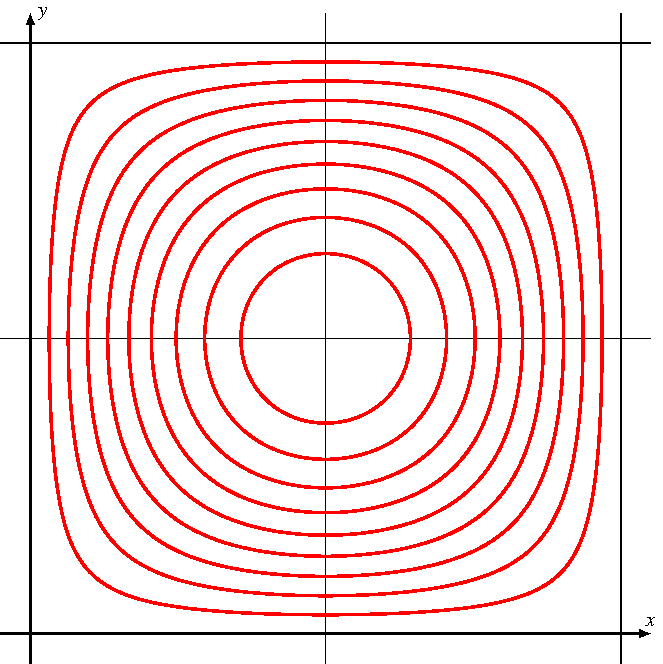
\includegraphics{chapters/2/konvektion.pdf}
\caption{Stromlinien in einer einzelnen Konvektionszelle
\label{skript:stromlinien konvektion}}
\end{figure}
Ausgehend von
\eqref{skript:lorenzausgangsgleichung}
versuchen wir nun, eine gewöhnliche Differentialgleichung zu gewinnen,
welche näherungsweise wiedergibt, was passiert, wenn im betrachteten
System Konvektion einsetzt.
Eine einzelne Konvektionszelle hat Stromlinien, wie sie in Abbildung
\ref{skript:stromlinien konvektion}
dargestellt sind.
Vernachlässigt man in der
ersten der Differentialgleichungen
\eqref{skript:lorenzausgangsgleichung}
$\vartheta$ und den nichtlinearen Term, bleibt eine Wärmeleitungsgleichung
für $\Delta \psi$
Die Wärmeleitungsgleichung auf einem Rechteckgebiet 
einer solchen Zelle könnte man mit einem Separationsansatz zu lösen
versuchen, dies würde auf Lösungen der Form
$\sin(ax)\sin(y)$
führen.
Wir versuchen daher eine Lösung für $\psi(x,y,t)$ in der etwas
allgemeineren Form
\begin{equation}
\psi(x,y,t)
=
X(t) \sin(ax)\sin(y)
\label{skript:psiansatz}
\end{equation}
zu finden.
Die Konvektion sorgt dafür, dass im Bereich grosser
Strömungsgeschwindigkeit der Temperaturgradient stark vom linearen Verlauf
abweicht.
Die vertikale Strömungsgeschwindigkeit ist bei $0$ und $\pi$ hoch, also
dort wo $\cos(ax)$ gross ist.
Wir setzen daher die Lösung für die Temperatur $\vartheta(x,y,t)$ an in der
Form
\begin{equation}
\vartheta(x,y,t)
=
Y(t) \cos(ax) \sin(y) - Z(t) \sin(2y).
\label{skript:thetaansatz}
\end{equation}
Das Ziel ist, für die drei Funktionen $X(t)$, $Y(t)$ und $Z(t)$
gewöhnliche Differentialgleichungen aufzustellen, also die Ortsabhängigkeit
der Lösungsfunktionen vollständig zu eliminieren.
Diese Technik heisst in der Theorie der partiellen Differentialgleichungen
auch die Transformationsmethode.

Wir können allerdings nicht erwarten, dass dies exakte Lösungen sind.
Beim Einsetzen in die Differentialgleichungen werden auch noch
andere Terme entstehen.
Unter der Annahme, dass die genannten Terme die Gestalt der Stromlinien
genau genug wiederzugeben in der Lage sind, vernachlässigen wir alle
Terme, die sich nicht als Vielfache der Funktionen
\begin{equation}
\sin(ax)\sin(y),
\qquad
\cos(ax)\sin(y)
\qquad\text{und}\qquad
\sin(2y)
\label{skript:funktionsauswahl}
\end{equation}
schreiben lassen.

Wir müssen jetzt also die Lösungsansatze
\eqref{skript:psiansatz}
und
\eqref{skript:thetaansatz}
in die Differentialgleichungen
\eqref{skript:lorenzausgangsgleichungen}
einsetzen.
Die linke Seite ist jeweils einfach, da die Zeitabhängigkeit nur noch
in den Funktion $X(t)$, $Y(t)$ und $Z(t)$ steckt.
Auf der linken Seite können wir daher einfach $X(t)$ durch $\dot X(t)$
ersetzen und analog für die anderen beiden Koeffizientenfunktionen.

Die Ortsableitungen geben etwas mehr zu tun:
\begin{align*}
\frac{\partial}{\partial x}\psi
&=
X(t)a\cos(ax)\sin(y)
&
\frac{\partial}{\partial y}\psi
&=
X(t)\sin(ax)\cos(y)
\\
\frac{\partial^2}{\partial x^2}\psi
&=
-X(t)a^2\sin(ax)\sin(y)
&
\frac{\partial^2}{\partial y^2}\psi
&=
-X(t)\sin(ax)\sin(y)
\\
\Delta\psi
&=-(a^2+1)\psi
&
\Delta^2 \psi
&=
(a^2+1)^2\psi.
\end{align*}
für $\psi$ und
\begin{align*}
\frac{\partial}{\partial x}\vartheta
&=
-aY(t) \sin(ax) \sin(y)
&
\frac{\partial}{\partial y}\vartheta
&=
Y(t) \cos(ax) \cos(y) - 2 Z(t)\cos(2y)
\\
\frac{\partial^2}{\partial x^2}\vartheta
&=
-a^2Y(t) \cos(ax) \sin(y)
&
\frac{\partial^2}{\partial y^2}\vartheta
&=
-Y(t) \cos(ax) \sin(y)
+4Z(t)\sin(2y)
\\
\Delta\vartheta
&=\mathrlap{-(a^2+1)Y(t)\cos(ax)\sin(y)+4Z(t)\sin(2y)}
\end{align*}
für $\vartheta$.
In den Differentialgleichungen brauchen wir aber noch die
Funktionaldeterminanten für die nichtlinearen Terme:
\begin{align*}
\frac{\partial(\psi,\Delta\psi)}{\partial(x,y)}
&=
\frac{\partial\psi}{\partial x} \frac{\partial\Delta\psi}{\partial y}
-
\frac{\partial\psi}{\partial y} \frac{\partial\Delta\psi}{\partial x}
=
-(a^2+1)\biggl(
\frac{\partial\psi}{\partial x} \frac{\partial\psi}{\partial y}
-
\frac{\partial\psi}{\partial y} \frac{\partial\psi}{\partial x}
\biggr)
=0
\\
\frac{\partial(\psi,\vartheta)}{\partial(x,y)}
&=
\frac{\partial\psi}{\partial x} \frac{\partial\vartheta}{\partial y}
-
\frac{\partial\psi}{\partial y} \frac{\partial\vartheta}{\partial x}
\\
&=
X(t)\biggl(
a \cos(ax)\sin(y)
\bigl(Y(t) \cos(ax) \cos(y) - 2Z(t)\cos(2y)\bigr)
\\
&\qquad
-
\sin(ax)\cos(y)
\bigl(-aY(t) \sin(ax) \sin(y) \bigr)
\biggr)
\\
&=
X(t)(a(\underbrace{\cos^2(ax)+\sin^2(ax)}_{\displaystyle=1})
Y(t)\underbrace{\sin(y)\cos(y)}_{\displaystyle{\textstyle\frac12}\sin(2y)}-2a\cos(ax)\sin(y)Z(t)\cos(2y))
\\
&=
\frac12aX(t)Y(t) \sin(2y)
-
2a X(t)Z(t) \cos(ax)\sin(y)\cos(2y)
\\
&=
\frac12aX(t)Y(t) \sin(2y)
-
2a X(t)Z(t) \cos(ax)\frac12(\sin(-y)+\sin(3y))
\\
&=
\frac12aX(t)Y(t) \sin(2y)
+
2aX(t)Z(t) \cos(ax)\sin(y)
-
2aX(t)Z(t) \cos(ax)\sin(3y).
\end{align*}
Der letzte Term kann nicht durch Funktionen aus der Liste
\eqref{skript:funktionsauswahl}
ausgedrückt werden, und muss daher vernachlässigt werden.
Setzen wir jetzt diese Ableitungen in die Differentialgleichungen
ein, erhalten wir
\begin{align*}
-(a^2+1)
\dot X(t) \sin(ax)\sin(y)
&=
\nu (a^2+1)^2 X(t)\sin(ax)\sin(y)
-acY(t)\sin(ax)\sin(y)
\\
\dot Y(t)\cos(ax)\sin(y)-\dot Z(t)\sin(2y)
&=
-\kappa (a^2+1)Y(t)\cos(ax)\sin(y) +4\kappa Z(t)\sin(2y)
\\
&\qquad +\frac{T_0}{\pi} X(t)a\cos(ax)\sin(y)
\\
&\qquad
-\frac{a}2X(t)Y(t)\sin(2y) - 2aX(t)Z(t)\cos(ax)\sin(y).
\end{align*}
Wir vergleichen die Koeffizienten der Funktionen aus der Liste
\eqref{skript:funktionsauswahl}
dann erhalten wir das Differentialgleichungssystem 

%(%i26)                               dglX
%             2       d                           4      2
%(%o26)   (- a  - 1) (-- (X(t))) + a c Y(t) + (- a  - 2 a  - 1) nu X(t)
%                     dt
%(%i27)                               dglY
%         a X(t) T_0   d                          2
%(%o27) - ---------- + -- (Y(t)) + a X(t) Z(t) + a  kappa Y(t) + kappa Y(t)
%            %pi       dt
%(%i28)                               dglZ
%                     d                          a X(t) Y(t)
%(%o28)             - -- (Z(t)) - 4 kappa Z(t) + -----------
%                     dt                              2

\begin{align*}
\dot X(t)
&=
-\nu(a^2+1)X(t)
+\frac{ac}{a^2+1}Y(t)
\\
\dot Y(t)
&=
\frac{aT_0}{\pi}X(t)
-(a^2+1)\kappa Y(t)
-aX(t)Z(t)
\\
\dot Z(t)
&=
-4\kappa Z(t)
+\frac{a}{2}X(t)Y(t)
\end{align*}
für die Koeffizientenfunktionen $X(t)$, $Y(t)$ und $Z(t)$.




\section*{Übungen}
\begin{uebungsaufgaben}
\item
Betrachten Sie die Differentialgleichung
\begin{equation}
\frac{dx}{dt}
=
x^4-4x^2-\lambda
\label{aufgabe301:gl}
\end{equation}
\begin{teilaufgaben}
\item
Finden Sie die Gleichgewichtslösungen und untersuchen Sie die 
Bifurkationen, die bei Veränderungen des Parameters $\lambda$
auftreten können.
\item
Welche Gleichgewichtslösung wird das System einnehmen, wenn der
Parameter $\lambda$ erst von $-1$ auf $1$ anwächst
und dann wieder auf $-1$ absinkt.
\end{teilaufgaben}

\begin{loesung}
\begin{figure}
\centering
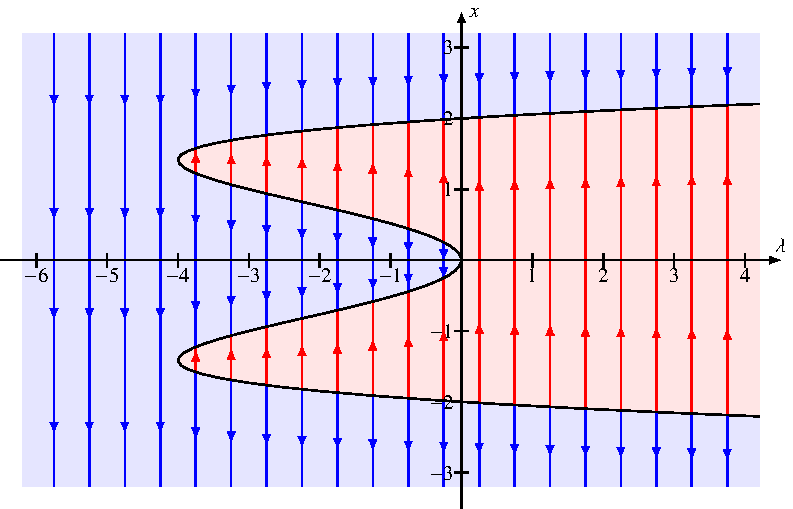
\includegraphics{chapters/3/grad4.pdf}
\caption{Phasendiagramm der Differentialgleichung~\eqref{aufgabe301:gl}.
\label{aufgabe301:fig}}
\end{figure}
\begin{teilaufgaben}
\item
Die kritischen Punkte der Differentialgleichung~\eqref{aufgabe301:gl}
sind Nullstellen der Gleichung
\begin{equation}
x^4-4x^2-\lambda=0
\label{aufgabe301:nullstellen}
\end{equation}
Dies ist eine quadratische Gleichung in $x^2$, die mit der Lösungsformel
für die quadratische Gleichung gelöst werden kann:
\[
x^2 = 2 \pm \sqrt{4+\lambda}.
\]
Diese Gleichung hat reelle Lösungen für $\lambda \ge -4$.
Für $\lambda \le 0$ ist die Quadratwurzel nicht grösser als $2$,
so dass die beiden Nullstellen positiv sind, es also vier verschiedene
Lösungen
\begin{equation}
x_{1,2,3,4} = \pm\sqrt{2\pm\sqrt{4+\lambda}}
\end{equation}
hat.
Für $\lambda >0$ hat die quadratische Gleichung eine negative Lösung
für $x^2$, die also nicht zu einer reellen Lösung der
Gleichung~\eqref{aufgabe301:nullstellen} führen kann.
Nur aus der positive Lösung $2+\sqrt{4+\lambda}$ kann man eine
Gleichgweichslösung, nämlich
\[
x=\pm\sqrt{2+\sqrt{4+\lambda}}
\]
ableiten.
Für $\lambda < -4$ gibt es gar keine Gleichgewichtslösung.

Das Phasendiagramm in Abbildung~\ref{aufgabe301:fig} zeigt,
dass für $\lambda >0$ die obere Gleichgewichtslösung stabil ist,
untere dagegen instabil.
Für $-4\le\lambda\le 0$ sind die Gleichgewichtslösungen
\begin{align*}
&\sqrt{2+\sqrt{4+\lambda}}
&&\text{und}&
&-\sqrt{2-\sqrt{4+\lambda}}
\\
\intertext{stabil und die Gleichgewichtslösungen}
&-\sqrt{2+\sqrt{4+\lambda}}
&&\text{und}&
&\sqrt{2-\sqrt{4+\lambda}}
\end{align*}
instabil.

Bei $\lambda=-4$ finden gleichzeitig zwei Sattel-Knoten-Bifurkationen 
statt, bei $\lambda=0$ findet ein einfache Sattel-Knoten-Bifurkation
statt, jedoch in umgekehrter Richtung wie im Beispiel im Text.
\item
Beim Anwachsen des Parameters über den Punkt $\lambda=0$ springt die
Gleichgewichtslösung auf die stabile Lösung
\[
x(\lambda)=\sqrt{2+\sqrt{4+\lambda}}.
\]
Bei der anschliessenden Verringerung von $\lambda$ bleibt die 
Gleichgewichtslösung auf dem Ast $x(\lambda)$ der Kurve, da diese
alle stabil sind.
Unabhängig vom Ausgangszustand befindet sich das System am Ende des
beschriebenen Szenarios also immer in der Nähe der Gleichgewichtslösung
\[
x(-1)=\sqrt{2+\sqrt{3}}.
\qedhere
\]
\end{teilaufgaben}
\end{loesung}


\end{uebungsaufgaben}


